% \textbf{\underline{OZ 3 - De Lorentzkracht en de wet van Ampère - Oefening 2:}}
% \vspace{0.5cm}

% Twee lange coaxiale solenoïdes dragen elke een stroom $ I $, maar in tegengestelde richting (Figuur 3.1). De binnenste spoel (straal $ a $) heeft $ n_1 $ wikkelingen per lengte-eenheid. De buitenste (straal $ b $) heeft er $ n_2 $. Bepaal $ \vec{B} $

% \begin{enumerate}[(a)]
%     \item in de binnenste spoel.
%     \item tussen de twee spoelen.
%     \item buiten de twee spoelen.
% \end{enumerate}

% \begin{figure}[H]
%     \centering
%     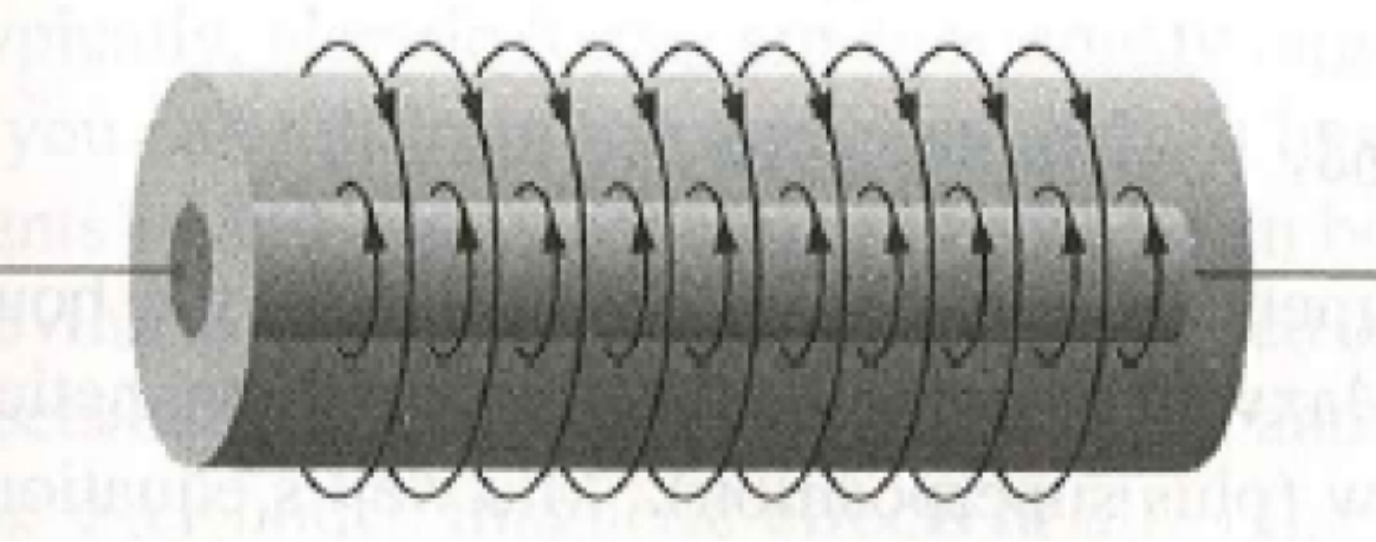
\includegraphics[width=7cm]{oz03/resources/oef-2-opgave.png}
    
%     \textbf{Figuur 3.1}
% \end{figure}

% \begin{description}[labelwidth=1.5cm, leftmargin=!]
%     \item[Geg. :]   $ I $; $ a $; $ n_1 $; $ b $; $ n_2 $;
% \end{description}

% \begin{enumerate}[(a)]
%     \item 
%         \begin{description}[labelwidth=1.5cm, leftmargin=!]
%             \item[Gevr. :]  $ \vec{B} $ in de binnenste spoel;
%             \item[Opl. :]   $ \vec{B} = \vec{B}_2 - \vec{B}_1 
%                             = \mu_0 n_2 I \hat{\imath} - \mu_0 n_1 I \hat{\imath}$
%         \end{description}
%     \item 
%         \begin{description}[labelwidth=1.5cm, leftmargin=!]
%             \item[Gevr. :]  $ \vec{B} $ tussen de twee spoelen;
%             \item[Opl. :]   $ \vec{B} = \vec{B}_2 - \vec{B}_1 
%                             = \mu_0 n_2 I \hat{\imath} - 0 
%                             = \mu_0 n_2 I \hat{\imath} $
%         \end{description}
%     \item 
%         \begin{description}[labelwidth=1.5cm, leftmargin=!]
%             \item[Gevr. :]  $ \vec{B} $ buiten de twee spoelen;
%             \item[Opl. :]   $ \vec{B} = \vec{B}_2 - \vec{B}_1  
%                             = 0 - 0
%                             = 0 $
%         \end{description}
% \end{enumerate}

% \vspace{1cm}